\subsection*{Операция Heapify}

\Def Heapify -- процесс построения кучи на заданном массиве. То есть
надо переупорядочить элементы в массиве так, чтобы по индексам на
всех парах родитель-сын было соблюдено свойство кучи.

\Solve Будем просеивать вниз элементы, начиная с $\frac{N}{2}$-го и до
нулевого.

\Proof 
Элементы с индексами больше $\frac{N}{2}$ не могут быть родителями в куче, значит изначально для них правило кучи не нарушается.
До вызова SiftDown для вершины, ее поддеревья являются кучами.
После выполнения SiftDown эта вершина с ее поддеревьями будут также являться кучей. 
Значит, после выполнения всех SiftDown получится куча. 
\Endproof

\Th Время работы данного алгоримта: O(n).

\Proof \\
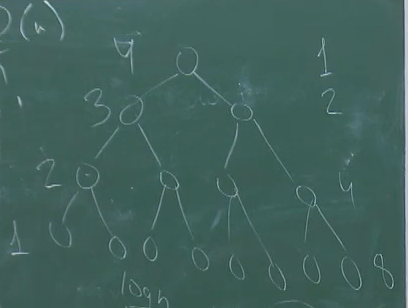
\includegraphics[width=5cm]{pix/25.png}

$\displaystyle\sum_{h=1}^{\log_{2}{n}} h*2^{\log_{2}{n} - h}$ = $n*\displaystyle\sum_{h=1}^{\log_{2}{n}} \frac{h}{2^h}$
 
$\displaystyle\sum_{h=1}^{\log_{2}{n}} \frac{h}{2^h}$ сходится к 2. Таким образом $T(n) = 2n$. Асимптотика O(n).
\Endproof

\begin{lstlisting}
void Heap::heapify() {
  for (int i = size / 2 - 1; i >= 0; --i) {
    siftDown(i);
  }
}
\end{lstlisting}

\subsection*{Пирамидальная сортировка}

\Task Отсортировать массив $a_1, \dots , a_n$ за $O(n\,log\,n)$ времени и $O(1)$ доппамяти.

\Solve 
\begin{enumerate}
    \item Выполнить Heapify.
    \item Пусть x = GetMin(), далее надо сделать ExtractMin() и вместо последнего элемента выписать x.
    \item Повторить это действие n - 1 раз.
    \item Развернуть массив.
\end{enumerate}

\pagebreak